%% BEGINING OF THE DOCUMENT
\documentclass[a4paper, 12pt]{article}

%% PACKAGE INCLUSION
\usepackage{color}
\usepackage{graphicx}
\usepackage[export]{adjustbox} 

%% BEGIN DOCUMENT
\begin{document}

%% TITLE AND HEADER
\title{PSG's Scratchpad for \LaTeX{}}
\author{Partha S. Ghosh}
\date{\today}
\maketitle

% TABLE OF CONTENTS
\pagenumbering{roman}
\tableofcontents
\newpage
\pagenumbering{arabic}

%\begin{abstract}
%This is a simple paragraph at the beginning of the 
%document. A brief introduction about the main subject.
%\end{abstract}
%\end{document}

%% SECTION 
\section{Introduction}
This is the introduction.
\section{Methods}
This is where methods starts.

%% SUBSECTION
\subsection{Stage 1}
\label{sec1}
This is where sub methods starts.
\subsubsection{Sub Sub Methods}
This is where sub sub methods starts.\\
There is no sub sub sub section.

\subsection{Stage 2}
This is the second part of the methods. I'm writing something here to test \footnote{footnotes working fine}
several features.
%\subsubsubsection{sub sub sub methods}
%This is where sub sub sub methods starts.

%% Reference and Page Reference
\section{Results}
Here are the results. Reffering to section \ref{sec1} on page \pageref{sec1}

\paragraph{This is the starting of the paragraph}


%% Typesetting Text
\section{Typesetting Text}
\subsection{Font Effects}
\textit{italics - a quick brown fox jumped over the lazy dog} \\
\textsl{slanted - a quick brown fox jumped over the lazy dog} \\
\textsc{smallcaps - a quick brown fox jumped over the lazy dog} \\
\textbf{bold - a quick brown fox jumped over the lazy dog} \\
\texttt{teletype - a quick brown fox jumped over the lazy dog} \\
\textsf{serif words - a quick brown fox jumped over the lazy dog} \\
\textrm{roman words - a quick brown fox jumped over the lazy dog} \\
\textup{uppercase - a quick brown fox jumped over the lazy dog} \\
\underline{underline - a quick brown fox jumped over the lazy dog}

\pagebreak
%%PAGE COLOR
\pagecolor{black}
\color{white}

\section{Coloured Text - a quick brown fox jumped over the lazy dog}
\subsection{Font Effects - a quick brown fox jumped over the lazy dog}
\textit{italics - {\color{red}a quick brown fox jumped over the lazy dog}} \\
\textsl{slanted - {\color{green}a quick brown fox jumped over the lazy dog}} \\
\textsc{smallcaps - {\color{blue}a quick brown fox jumped over the lazy dog}} \\
\textbf{bold - {\color{yellow}a quick brown fox jumped over the lazy dog}} \\
\texttt{teletype - {\color{cyan}a quick brown fox jumped over the lazy dog}} \\
\textsf{serif words - {\color{magenta} quick brown fox jumped over the lazy dog}} \\
\textrm{roman words - a quick brown fox jumped over the lazy dog} \\
\textup{uppercase - a quick brown fox jumped over the lazy dog} \\
\underline{underline - a quick brown fox jumped over the lazy dog}

\pagebreak
%% ENDING PAGE COLOR
\pagecolor{white}
\color{black}
\subsection{Font Size}
{\tiny time: a quick brown fox jumped over the lazy dog.}\\
{\scriptsize scriptsize: a quick brown fox jumped over the lazy dog.}\\
{\footnotesize footnotesize: a quick brown fox jumped over the lazy dog.}\\
{\small small: a quick brown fox jumped over the lazy dog.}\\
{\normalsize normalsize: a quick brown fox jumped over the lazy dog.}\\
{\large large: a quick brown fox jumped over the lazy dog.}\\
{\LARGE LARGE: a quick brown fox jumped over the lazy dog.}\\
{\Large Large: a quick brown fox jumped over the lazy dog.}\\
{\huge huge: a quick brown fox jumped over the lazy dog.}\\
{\Huge Huge: a quick brown fox jumped over the lazy dog.}\\


%% LISTS
\section{Lists}
Lists are of two types. \textbf{enumerate} produces numbered lists while \textbf{itemize} is for bulleted lists.
\subsection{Enumerated Lists}
\begin{enumerate}
\item First thing
\item Second thing
\item Third thing
\item Fourth Thing
\end{enumerate}

\subsection{itemized lists}
\begin{enumerate}
\item First thing
\begin{itemize}
\item First First item
\item First Second item
\end{itemize}
\item Second thing
\begin{itemize}
\item[-] Second First item
\item[-] Second Second item
\end{itemize}
\item Third thing
\begin{itemize}
\item[*] Second First item
\item[*] Second Second item
\end{itemize}
\item Fourth Thing
\begin{itemize}
\item[+] Second First item
\item[+] Second Second item
\end{itemize}
\end{enumerate}

\section{Comments \& Spacing}
Comments are created using \% \\

Special characters are printed as \\
\# \\
\$ \\
\% \\
\^{} \\
\& \\
\_ \\
\{ \\
\} \\
\~{} \\
\textbackslash \\

\textit{Look at \textbf{LaTeX\_symbols.pdf} for more details on the fonts}

\section{Tables}
The \textsf{tabular} command is used to typeset tables.\\

\begin{tabular}{|l|l|}
Apples & Green\\
Strawberries & Red \\
Oranges & Orange \\
\end{tabular} \\

Next Table with horizontal line\\

\begin{tabular}{|l|l|}
\hline
Apples & Green\\
\hline
Strawberries & Red \\
\hline
Oranges & Orange \\
\hline
\end{tabular} \\

Next Table \\

\begin{tabular}{|r|l|}
\hline
8 & here's \\
\cline{2-2}
86 & stuff \\
\hline \hline
2008 & now \\
\hline
\end{tabular} \\

Table \ref{table:data} is an example of referenced \LaTeX{} elements. \\

\begin{table}[h!]
\centering
\begin{tabular}{||c c c c||} 
 \hline
 Col1 & Col2 & Col2 & Col3 \\ [0.5ex] 
 \hline\hline
 1 & 6 & 87837 & 787 \\ 
 2 & 7 & 78 & 5415 \\
 3 & 545 & 778 & 7507 \\
 4 & 545 & 18744 & 7560 \\
 5 & 88 & 788 & 6344 \\ [1ex] 
 \hline
\end{tabular}
\caption{Table to test captions and labels}
\label{table:data}
\end{table}

\section{Figures}
\begin{figure}
\centering
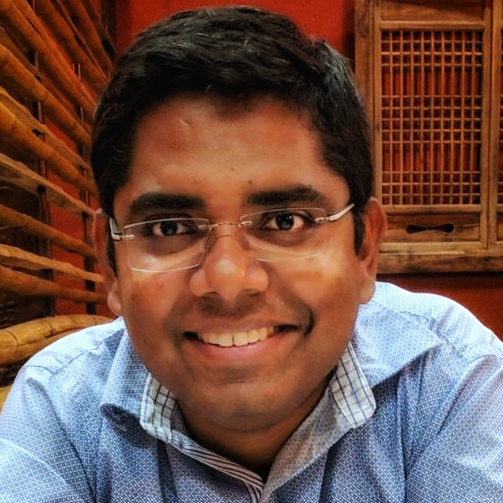
\includegraphics[max size={\textwidth}{\textheight}]{myimage.jpeg}
\caption{Partha Ghosh Image}
\label{psgimg}
\end{figure}

\section{Figures}
\begin{figure}
\centering

\includegraphics{mohunBagan.png}
\caption{Mohun Bagan}
\label{mbimg}
\end{figure}

\section*{Unnumbered Section}
This is an unnumbered section

% a quick brown fox jumped over the lazy dog \\
% A QUICK BROWN FOX JUMPED OVER THE LAZY DOG \\
\end{document}